\chapter{Molecular Imaging methods}
\label{sec:imaging}

In current chapter molecular imaging methods \textit{computed tomography} and 
\textit{cryo-electron microscopy} (cryo-EM) will be introduced. 
Further, their observation model is defined in a mathematic way and reconstruction is presented.
Application of cryo-EM is a major motivation for the Master Thesis, 
as the problem is not easy to solve due to dealing with enormous noise and unknown observation angles.
Computed Tomography is a similar problem and is therefore well suited as a
first step to make an algorithm work for cryo-EM. 


\section{Computed tomography}
Computed tomography (CT) is a well established molecular imaging method.
Using X-ray source, fan shaped beams are produced which scan the imaging object,
resulting in many observations taken over straight lines \cite{computedTomography}.

\paragraph{Tomography reconstruction:}
Tomographic reconstruction \cite{tomographicReconstruction} is a popular inverse problem. 
The aim is to reconstruct an imaged object from observed observations.
The reconstruction object can be in two-dimension (2D) or in three-dimension (3D). 

\begin{tcolorbox}[colback=red!5!white,colframe=red!75!black]
    The focus in computed tomography during the Thesis will be on 2D case, which is called \textit{classical tomography reconstruction}.
\end{tcolorbox}

\paragraph{2D tomographic reconstruction:}

Mathematically, observations are defined as follows:
\begin{equation}
    \label{eq:2Dreconstruction}
    \begin{aligned}
        y_i[j] &= p_i + \eta_i[j] , \text{ with } 1 \leq i \leq N \text{ and } 1 \leq j \leq M, \\
        y_i[j] &= R(x, \theta_i, s_j) + \eta_i[j] , \text{ with } 1 \leq i \leq N \text{ and } 1 \leq j \leq M,
    \end{aligned}
\end{equation}

with
\begin{itemize}
    \item $N$: number of observations
    \item $M$: observation dimension
    \item $y_i \in \mathbb{R}^M$:  $i$-th observation with $y_i[j] \in \mathbb{R}$: $j$-th element of observation
    \item $p_i \in \mathbb{R}^M$:  $i$-th noiseless observation with $p_i[j] \in \mathbb{R}$: $j$-th element of observation
    \item $x \in L^2(\Omega)$: original object with $\Omega \subset \mathbb{R}^2 $ and $L^2$: Lebesgue space
    \item $R(\cdot; \theta, s): L^2(\Omega) \to L^2(\tilde{\Omega}) , x \mapsto R(x; \theta,s)$: Radon Transform \cite{radonTransform} with,\\
        $\tilde{\Omega} \subset \mathbb{R}$, $\theta_i \in \mathbb{R}$: observation angle and $s_j \in \mathbb{R}$: sampling point 
    \item $\eta_i \in \mathbb{R}^M$: gaussian noise with $\eta_i[j] \sim \mathcal{N}(0,\sigma^2) \in \mathbb{R}$
\end{itemize}

\begin{tcolorbox}[colback=red!5!white,colframe=red!75!black]
    During Thesis, the notation $p$ for noiseless observation and $y$ for observation with noise is used.
    In practise, $p$ is not observable directly and the observed signal $y$ needs to be denoised.
    Further, $x$ is used for original object.
\end{tcolorbox}

% where $y_i \in \mathbb{R}^M$ is $i$-th observation with $y_i[j] \in \mathbb{R}$ $j$-th element of the observation
% and $M$ the observation dimension. 
% Further, $N$ corresponds to number of observations.

% Then, $x \in L^2(\Omega)$ is the original object with $\Omega \subset \mathbb{R}^2 $ and $L^2$ the Lebesgue space.

% $R(\cdot; \theta, s): L^2(\Omega) \to L^2(\tilde{\Omega}) , x \mapsto R(x; \theta,s)$ refers to the Radon Transform \cite{radonTransform} 
% with $\tilde{\Omega} \subset \mathbb{R}$, $\theta_i \in \mathbb{R}$ as observation angle and $s_j \in \mathbb{R}$ 
% as sampling point. Finally, $\eta_i \in \mathbb{R}^M$ refers to gaussian noise and 
% is defined as $\eta_i[j] \sim \mathcal{N}(0,\sigma^2) \in \mathbb{R}$.
Data of Radon Transform is often called a \textit{sinogram}.
In figure~\ref{fig:phantom} the Shepp-Logan phantom can be seen. 
It is often used as an image for simulating a brain CT.
Further, in figure~\ref{fig:phantom_sinogram} and figure~\ref{fig:phantom_sinogram_noisy} 
observation sinograms can be seen with and without noise respectively. 
To apply Radon Transform, parameter $\theta$ and $s$ need to be specified.
In this case, $\theta \in \mathbb{R}^{500}$ was evenly spaced
between $[0, 2 \pi]$ and $s$ was set to $400$, which is the Shepp-Logan phantom image resolution
and results in one observation per pixel.
Further, noise was added to reach a signal-to-noise-ratio (SNR) of 10dB.

\begin{figure}[H]
    \label{fig:phantom_and_sinos}
    % \centering
    \hfill
    \subbottom[Shepp-Logan phantom: $x$ \label{fig:phantom}]{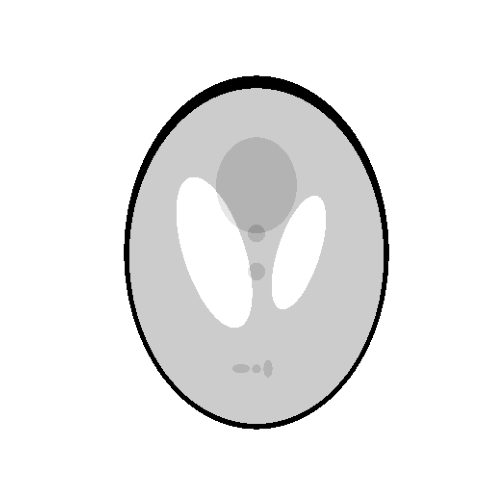
\includegraphics[width=0.22\textwidth]{phantom.png}}
    \hfill
    \subbottom[Clean Sinogram: $R(x, \theta, s) = p$   \label{fig:phantom_sinogram}]{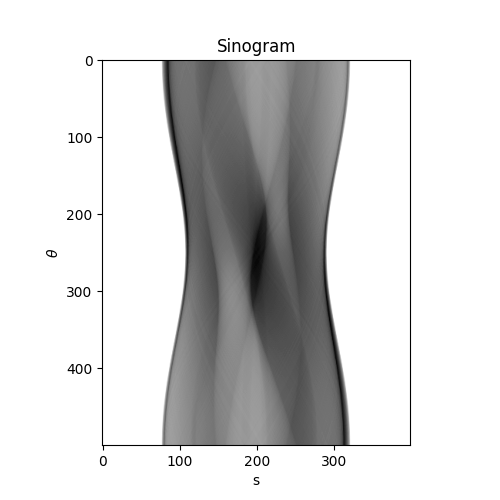
\includegraphics[width=0.22\textwidth]{phantom_sino.png}}
    \hfill
    \subbottom[Noisy sinogram: $R(x, \theta, s) + \eta = y + \eta$ \label{fig:phantom_sinogram_noisy}]{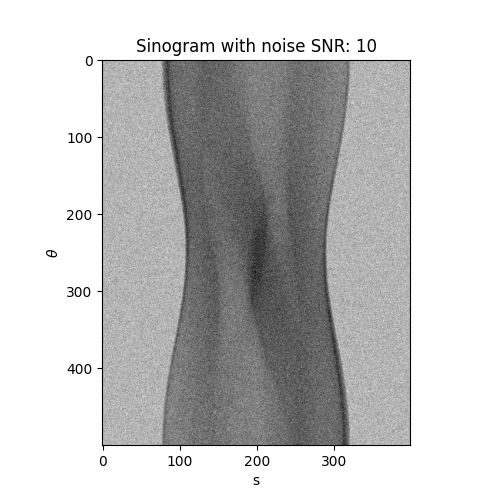
\includegraphics[width=0.22\textwidth]{phantom_sino_noisy_snr10.png}}
    \hfill
	\caption{Shepp-Logan phantom and sinogram}
\end{figure}

\subparagraph{Filter Backprojection:}
Filter Backprojection \cite{tomographicReconstruction} (FBP), 
is a reconstruction method, typically used in classical tomography.
It allows to inverse the Radon Transform and enables reconstruction of the original object $x$.
It can be defined as:

\begin{equation}
    \label{eq:fbp}
    FBP(\cdot; \theta, s) : L^2(\tilde{\Omega}) \to L^2(\Omega), y \mapsto FBP(y; \theta, s) ,
\end{equation}

with $\theta$ as projection angle and $s$ sampling points. 
The algorithm fails when working with noisy data \cite{cryoEmMath2}.

\begin{figure}[H]
    \label{fig:phantom_fbps}
    % \centering
    \hfill
    \subbottom[Clean reconstruction: $FBP(p, \theta, s)$  \label{fig:fbp_phantom}]{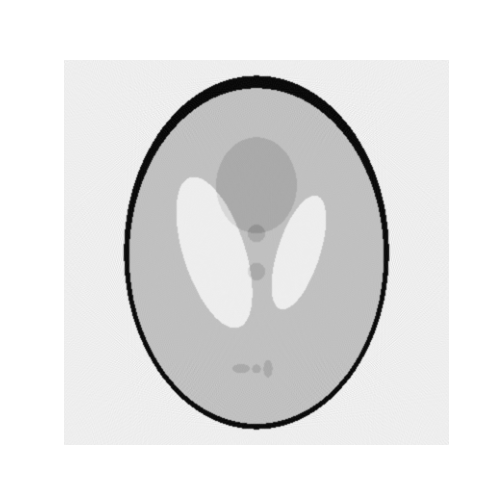
\includegraphics[width=0.22\textwidth]{fbp_phantom_clean.png}}
    \hfill
    \subbottom[Noisy reconstruction: $FBP(y, \theta, s)$ \label{fig:fbp_phantom_noisy}]{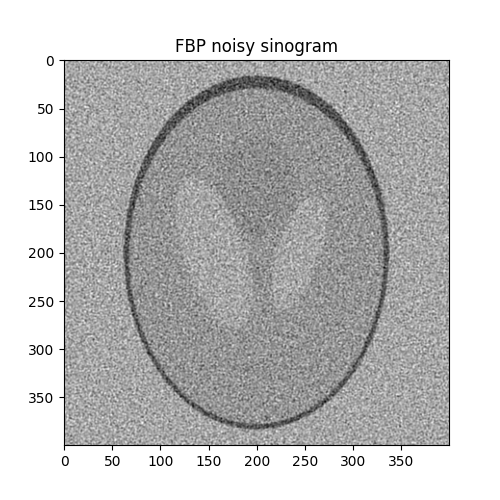
\includegraphics[width=0.22\textwidth]{fbp_phantom_snr_10.png}}
    \hfill
	\caption{Shepp-Logan sinograms and filter-back projection reconstructions}
\end{figure}

In figure~\ref{fig:fbp_phantom} and figure~\ref{fig:fbp_phantom_noisy} reconstruction using FBP can be seen from 
Shepp-Logan phantom sinogram (figure~\ref{fig:phantom_sinogram}) and its noisy version (figure~\ref{fig:phantom_sinogram_noisy}).

\subparagraph{U-Net}
\ref{ct-reconstruction-comparison} compared different reconstruction methods for computed tomography. 
Deep Learning approaches have great potential in CT reconstruction and \ref{unet-tomography} performed much better than FBP.
\textbf{TODO: Few words about how u-net works}
\textbf{TODO: Add some figures with final u-net pre trained model.}

\section{Cryo-EM}
Cryo-EM is another molecular imaging method, that enables the view of molecules in near-atomic resolution.
In the Master Thesis, only single-particle cryo-EM \cite{singleParticleCryoEm} is considered, 
when writing about cryo-EM it always refers to single-particle cryo-EM.

During imaging process molecules are frozen in a thin layer of ice, where they are randomly oriented and positioned. 
Random orientation and positioning makes reconstruction challenging, 
but freezing allows observation in a stable state where molecules are not moving.
With an electron microscope, two-dimensional tomographic projection images of molecules in the ice are observed,
which are called \textit{micrograph}. 
Frozen molecules are fragile and electron microscope needs to work with
very low power (electron dose), resulting in highly noisy images. The resulting (SNR)
is typically smaller than 1, which indicates that there is more noise than signal \cite{cryoEmMath2}.

Further, observed molecules are not equal in the sense that there are some structural varieties between
molecules (isotopes). Wile observing the same molecule in ice many times, single observation could be from different isotopes.

\paragraph{3D cryo-EM reconstruction:}
Similar to tomographic reconstruction, cryo-EM reconstruction problem \cite{cryoEmMath} is defined.
It can be seen as a 3D reconstruction problem as the original object $x \in L^2(\Omega)$ to be reconstructed is in 3D.
Based on many observed micrographs, collected by the electorn microscope, the original object $x$ will be estimated.

Cryo-EM reconstruction is computational intensive and multiple steps are needed to get from observed, raw data to the final structure \cite{singleParticleCryoEm}.

Mathematically, observation is defined as follows:
\begin{equation}
    \label{eq:cryoEmSimple}
    \begin{aligned}
        y_i &= p_i + \eta_i, \text{ with } 1 \leq i \leq N,\\
        y_i &= \Pi_z  (\; Rot (\;x; \theta_i )) + \eta_i, \text{ with } 1 \leq i \leq N,    
    \end{aligned}
\end{equation}

where 
\begin{itemize}
    \item $N$: number of observations
    \item $M$: observation dimension
    \item $y_i \in \mathbb{R}^M$:  $i$-th observation with $y_i[j] \in \mathbb{R}$: $j$-th element of observation
    \item $p_i \in \mathbb{R}^M$:  $i$-th noiseless observation with $p_i[j] \in \mathbb{R}$: $j$-th element of observation
    \item $x \in L^2(\Omega)$: original object with $\Omega \subset \mathbb{R}^3 $ and $L^2$: Lebesgue space
    \item $\Pi_z : L^2(\Omega) \to L^2(\tilde{\Omega}), x \mapsto  \int x(\cdot,\cdot,z) dz$: Z-axis projection operator,
          with $\tilde{\Omega} \subset \mathbb{R}^2$
    \item $\theta_i = [\theta_i^{(1)}, \theta_i^{(2)}, \theta_i^{(3)} ] $: 3D rotation matrix with $ \theta_i^{(1)}, \theta_i^{(2)}, \theta_i^{(3)} \in \mathbb{R}$ and \\
          $R_{\theta_i} =  R_{e_x} (\theta_i^{(1)}) R_{e_y} (\theta_i^{(2)}) R_{e_z} (\theta_i^{(3)}) = [R^1_{\theta_i}, R^2_{\theta_i}, R^3_{\theta_i}] \in SO(3)$ \\
          (see \ref{app:3DrotationMatrix} for further details)
    \item $Rot : L^2(\Omega) \to L^2(\Omega), Rot(x, \theta_i) = \left((x_1,x_2,x_3) \mapsto x( x_1R^1_{\theta_i}, x_2R^2_{\theta_i}, x_3R^3_{\theta_i})\right)$: rotation operator
    \item $\eta_i \in \mathbb{R}^M$: gaussian noise with $\eta_i[j] \sim \mathcal{N}(0,\sigma^2) \in \mathbb{R}$
\end{itemize}

% $y_i \in \mathbb{R}^M$ with $M$ as observation dimension.

% Then, $\Pi_z : L^2(\Omega) \to L^2(\tilde{\Omega}), x \mapsto  \int x(\cdot,\cdot,z) dz$ is projection operator from z-axis
% and $Rot : L^2(\Omega) \to L^2(\Omega), Rot(x, \theta_i) = \left((x_1,x_2,x_3) \mapsto x( x_1R^1_{\theta_i}, x_2R^2_{\theta_i}, x_3R^3_{\theta_i})\right)$ is rotation operator modelling the rotation during freezing.
% Further, $\theta_i = [\theta_i^{(1)}, \theta_i^{(2)}, \theta_i^{(3)} ] $ where entries $ \theta_i^{(1)}, \theta_i^{(2)}, \theta_i^{(3)} \in \mathbb{R}$ and 
% $R_{\theta_i} =  R_{e_x} (\theta_i^{(1)}) R_{e_y} (\theta_i^{(2)}) R_{e_z} (\theta_i^{(3)}) = [R^1_{\theta_i}, R^2_{\theta_i}, R^3_{\theta_i}] \in SO(3)$ is the 3D rotation matrix 
% (see \ref{app:3DrotationMatrix} for further details). 
% $\eta_i \sim \mathcal{N}(0,\sigma^2I) \in \mathbb{R}^M$ corresponds to noise of observation.


As $y_i$ is not observable directly, discretization is needed:
\begin{equation}
    \label{eq:cryoEmSimpleDiscrete}
    \begin{aligned}
        y_i &= \left( \Pi_z (\; Rot (\;x; \theta_i)) + \eta_i\right)(\Delta), \text{ with } 1 \leq i \leq N \\
        y_i[j,k] &= \Pi_z (\; Rot(\;x; \theta_i))_{j,k} + \eta_i[j,k], \text{ with } 1 \leq i \leq N \text{ and } 1 \leq j,k \leq M,
    \end{aligned}
\end{equation}

where 
\begin{itemize}
    \item $\Delta \subset \tilde{\Omega}^{M^2}$: sampling grid with dimension $M^2$
    \item Further, $y[j,k]$, $\eta[j,k]$ and $\Pi_z(\cdot)_{j,k}$ $ \in \mathbb{R}$ with $j,k$ as indices of the sampling grid.
\end{itemize}
% $\Delta \subset \tilde{\Omega}^{M^2}$ is the sampling grid with dimension $M^2$.
% Further, $y[j,k]$, $\eta[j,k]$ and $\Pi_z(\cdot)_{j,k}$ $ \in \mathbb{R}$ with $j,k$ as indices of 
% the sampling grid.


\begin{figure}[H]
    \label{fig:cryo-em-omicron}
    % \centering
    \hfill
    \subbottom[COVID-19 Omicron spike: $x$ \label{fig:omicron}]{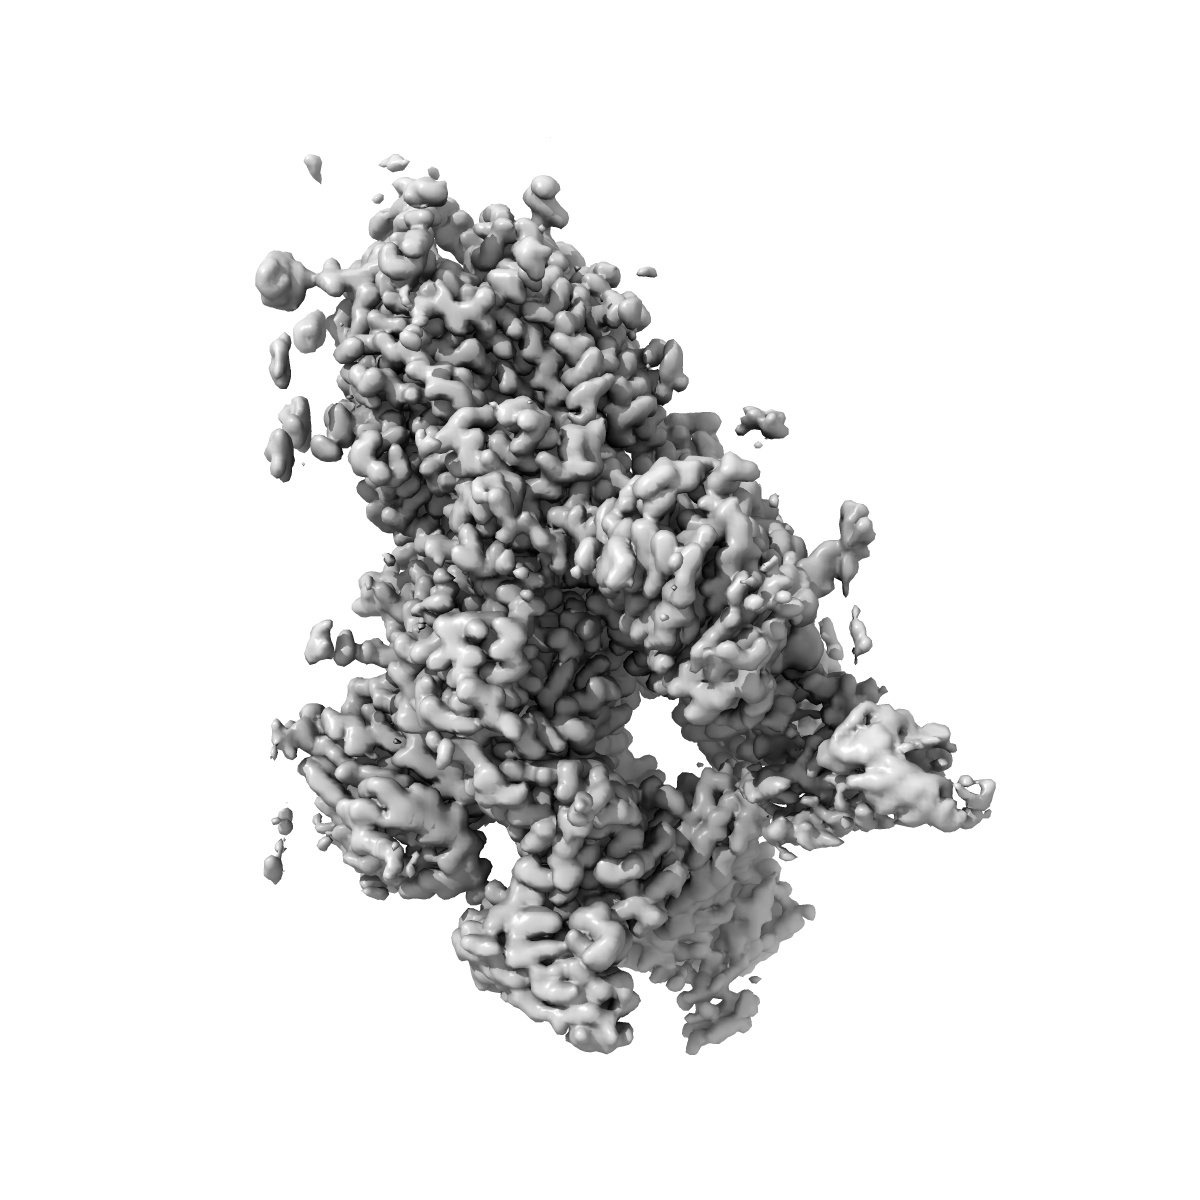
\includegraphics[width=0.18\textwidth]{emd_32500.map_xsurface.jpeg}}
    \hfill
    \subbottom[Projection along X-Axis: $p_1$   \label{fig:omicron-x}]{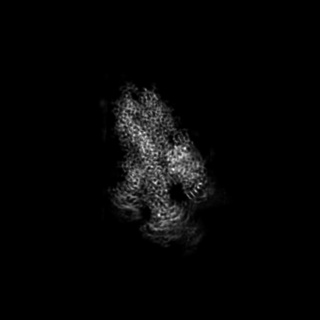
\includegraphics[width=0.18\textwidth]{emd_32500.map_xprojection.jpeg}}
    \hfill
    \subbottom[Projection along Y-Axis: $p_2$  \label{fig:omicron-y}]{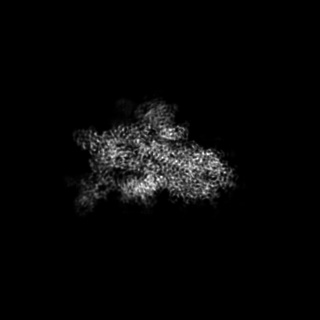
\includegraphics[width=0.18\textwidth]{emd_32500.map_yprojection.jpeg}}
    \hfill
    \subbottom[Projection along Z-Axis: $p_3$   \label{fig:omicron-z}]{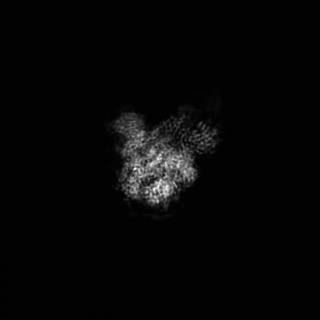
\includegraphics[width=0.18\textwidth]{emd_32500.map_zprojection.jpeg}}
    \hfill
	\caption{Cryo-EM reconstruction and clean projections of COVID-19 Omicron spike \protect\footnote{https://www.ebi.ac.uk/emdb/EMD-32500}}
\end{figure}


\subparagraph{Extended formula:} 
Equation~\ref{eq:cryoEmSimple} is a simplified version of cryo-EM.
First of all, point spread function (PSF) of the microscope is not taken into account.
Secondly, structural variety is ignored, the underlying object $x$ is not the same 
for every observation as modelled in the equation. 
Precisely, $x$ can be seen as a random signal from an unknown distribution defined over all possible molecules structures.

The equation can be extended and defined as the following:
\begin{equation}
    \label{eq:cryoEmExtended}
    y_i = h_i \circ \Pi_z ( Rot (x_i; \theta_i)) + \eta_i, \text{ with } 1 \leq i \leq N
\end{equation}

where $h_i$ is the PSF of the microscope and $\circ$ defines the convolution.
Further, $x_i \in X$ where $X$ is the set of all possible molecule structures.


\subparagraph{Difference to tomographic reconstruction:}
The problems are highly related, but cryo-EM reconstruct is more challenging.
While CT observation, patient is asked to not move and therefore, angles of projection are known.
Whereas, in cryo-EM this information will be lost during freezing.
Secondly, high level of noise makes cryo-EM much more challenging.


\section{Abstract form}
As tomographic reconstruction and cryo-EM reconstruction are rather similar, 
goal of the Master Thesis will be to design an algorithm, that can be applied in both scenarios.

Therefore, an abstract form of the problems will be defined in the following.
First of all, a similar notation as before is used, but in a more general way with
$x \in L^2(\Omega)$ where $\Omega \subset \mathbb{R}^D$ with $D$ as the dimension of the space of original object
and $\tilde{\Omega} \subset \mathbb{R}^{D-1}$ as the dimension of the space of observations.


\begin{equation}
    \begin{aligned}
        y_i &= p_i + \eta_i (\Delta), \text{ with } 1 \leq i \leq N \\
        y_i &= \left( A(x, \theta_i) + \eta_i \right) (\Delta), \text{ with } 1 \leq i \leq N 
    \end{aligned}
\end{equation}
with, 
\begin{itemize}
    \item $N$: number of observations
    \item $M$: observation dimension
    \item $y_i \in \tilde{\Omega}^M$: the $i$-th observation
    \item $p_i \in \tilde{\Omega}^M$: the $i$-th noiseless observation
    \item $x \in L^2(\Omega)$: original object
    \item $A: L^2(\Omega) \to L^2(\tilde{\Omega}), x \mapsto A(x; \theta_i)$: a non-linear operator 
    \item $\theta_i \in \mathbb{R}^P$: projection angle vector with $P$ the projection dimension
    \item $\eta \sim \mathcal{N}(O, \sigma^2 I) \in \tilde{\Omega}^M$: gaussian noise
    \item $\Delta \subset \tilde{\Omega}^{M}$: term for discretization
\end{itemize}

Further, an abstract form of the reconstruction operator is defined as 
\textbf{TODO: Abstract from of reconstruction}

\begin{equation}
    Recon : L^2(\tilde{\Omega}) \to L^2(\Omega), y \mapsto Recon(y; \theta_i)
\end{equation}



\paragraph{Classical tomography reconstruction:}

Classical tomography parameters are defined with $D=2$, $P=1$.
Further, $A(\cdot)$ is the Radon Transform (see equation~\ref{eq:2Dreconstruction}).
A distance measure between observations can be set up by using the $\ell2$-norm $\norm{y_i - y_j}$.

\paragraph{Cryo-Em reconstruction:}
Cryo-EM parameters are defined with $D=3$ and $P=3$ as $\theta_i$ not only corresponds to
a projection angle vector but also some rotation.
Further, $A(\cdot)$ can be defined as $\Pi_z \left(\; Rot(\;x; \theta) \right)$ 
where $Rot$ is the 3D rotation and $\Pi_z$ the tomographic projection (see equation~\ref{eq:cryoEmSimpleDiscrete}).

As observations are drawn with some random 3D rotation and projection, 
it can happen that two samples are equivalent up to 2D rotation. 
Consider a first observation $y_1$, which has no 3D rotation and 
a second observation $y_2$ with a rotation in x-y plane by 45°.
The two observations have a defined in-plane rotation $g$, such that $g \; y_1 = y_2$.
Therefore, a term of in-plan rotation is added to the $\ell2$-norm: $min_{g \in SO(1)}\norm{g \;y_i - y_j}$, 
which is inspired by \cite{multiDiffusionMaps}. 

\paragraph{High noise regime:}
Cryo-EM observations are highly noisy, which makes reconstruction challenging. 
There are different ways to reduce noise from observations, most of them are related to averaging. 
Averaging need to consider similar observations and ignore diverse ones. 
In the defined abstract model, averaging over paired observations from $\theta$ should be a good averaging model.
But how can it be achieved? 

One idea would be to measure distances between observation.
Another way is to find a low-dimensional embedding which maps our observations $y$ to some $\theta$.
When talking from low-dimensional embeddings, there is no way around Graph Learning, which will be introduced
in the following chapter~\ref{sec:graphFoundations}.

% \begin{tcolorbox}[colback=red!5!white,colframe=red!75!black]
%     During the Master Thesis, high-noise regime is domain of interest.
%     Main practical application is cryo-EM, where an algorithm for denoising is expected to boost
%     quality of the overall 3D-reconstruction. As cryo-EM is a 3D problem, computed tomography will
%     be considered as well which allows to test on a corresponding 2D problem.
%     The goal of the Master Thesis is to introduce a denoising algorithm, which is able to work well even 
%     on highly noisy data. Reconstruction of original object is not in the scope of the project.
% \end{tcolorbox}
